\section{Backgrounds (P2)}\label{sec:bkg}

Any two straight lines through the primary vertex are coplanar with it, and at pile-up 200 the inner tracker contains
$\sim10^5$ hits per event, so coplanar patterns arise both from random combinations of pile-up hits and from SM
topologies with a vertex on a line through the PV. This section describes how each background term of
Eq.~\eqref{eq:bsum} is estimated. The methods are pre-registered (\rep{plan.md} \S4, \rep{WP_RULE.md} \S4, \S6, \S7);
the numbers are from the final analysis run (C12FC\_v1, \rep{acts/stage4/STAGE4_RESULTS.md} \S1--3).

\subsection{Pile-up-only fake rate}\label{sec:bkg:pu}
A WP needs a pile-up fake probability of order $10^{-9}$ per triggered event, while a direct measurement would need
$\gtrsim10^9$ simulated pile-up events. The probability is therefore measured directly where possible and extrapolated
otherwise, by two pre-registered methods.
\begin{itemize}
\item \textbf{Direct ladder} (sample B1): pile-up-only events at the normalised density ($\rho=1$), each searched in four MET
  roads $\pi/2$ apart with a PV drawn from the luminous region independently of the pile-up vertices. The per-trial rate
  (mean over roads) is the primary estimator, because a data event has exactly one MET road.
\item \textbf{Interaction-count thinning} (sample B2): pile-up at $\rho=1$ is exactly a Poisson thinning, keeping each
  interaction with probability $q=1/\rho$, of the superposition of $\rho$ independent normalised events. For a candidate
  found at density $\rho$ whose in-band hits come from the interaction set $S$, the expected number of passing candidates
  at $\rho=1$ is weighted by
  \begin{equation}
    w_r=\sum_{T\subseteq S\ \text{passes}\ r} q^{|T|}(1-q)^{|S|-|T|},
    \label{eq:thinning}
  \end{equation}
  computed exactly by a per-layer dynamic programme for the counting rungs and by conditional importance sampling for
  the per-subset rungs. A candidate needing $n_{\rm int}$ specific interactions enters with $\rho^{-n_{\rm int}}$, so the
  method reaches deep into the tail without a fitted exponent; each top-up crossing counts as its own interaction.
  Candidates are counted once per distinct passing hit set (sets sharing $\ge50\%$ of their hits are one).
  Check of Eq.~\eqref{eq:thinning}: for $q=1$ it returns the pass indicator of the full set (verified on 2000 sets).
\item \textbf{Rung factorisation} beyond the reach of both: conditional pass fractions measured on the tightest population
  with at least ten entries, with a pre-registered factorisation (independence) test whose correlation factor
  multiplies the estimate if it exceeds one at $2\sigma$.
\end{itemize}

\subsection{Closure of the extrapolation and the seed threshold}\label{sec:bkg:closure}
The thinning prediction from $\rho=2$ is tested against the direct $\rho=1$ count at the deepest rung where both have
statistics (test T1 at R04, T1w at the first width rung), with the pre-registered criterion $|z|<2$. In the G3 pilot
(127 of 130 pile-up-only jobs) the test \textbf{failed in the anti-conservative direction} ($N_{\rm obs}/N_{\rm pred}=1.32$,
$z=+14.3$, for T1; 1.42, $z=+17.6$, for T1w; over-merging of hit sets at $\rho=2$). By user decision the pre-registered
conservative end state applies: the pile-up estimate is multiplied by the observed factors (compounded at deeper rungs),
the trend enters $\sigma_{\ln}$, and the closure is re-measured in production. The pilot also triggered the pre-declared
action $\Tseed:=4$ (pass fraction moved by more than $2\sigma$ between $\Tseed=6$ and 4).
On the production samples at $\Tseed=4$ (B1: 48\,000 trials; B2: 6000 trials) the closure is again
anti-conservative: $N_{\rm obs}/N_{\rm pred}=1.500$ ($z=+52.8$) for T1 at R04 and 1.606 ($z=+59.4$) for T1w at R05 (the
lever-arm requirement fails at R06). The compounded factor $\times2.41$ multiplies the pile-up estimate at every rung
from R05 on, and the significant downward trend of the ratio along R04--R07 ($-0.36$ per rung) enters only
$\sigma_{\ln}$, linearly in the rung index. The $dE/dx$ closure test is untestable (fewer than ten counts) and the
factorisation test is degenerate, so \textbf{beyond R06 (the deepest rung with ten counts at $\rho=2$; R07 for the direct
B1 count) the pile-up estimate rests on rung factorisation without an informative cross-variable closure test}. The
thinning reach is $\approx1.7\times10^{-10}$ per trial (\EST{}), against $\approx2.7\times10^{-10}$ that the pile-up term
alone would need to fill the whole SR-G budget: the reach would suffice in principle, but the deepest rung with at least
ten $\rho=2$ counts is R06. The $\sigma_{\ln}$ of the pile-up term is dominated by the density
normalisation (1.15--1.89) at loose rungs and, from R11 on, by the trend term (2.0 to 6.3) and the spread between
extrapolation models (4.76); the F1 helix and opening variables pass every pile-up record and earn no credit.

\subsection{SM hard-scatter backgrounds and normalisation}\label{sec:bkg:sm}
Two prompt tracks from the PV are coplanar with it; $W\to\tau\nu$ with a three-prong $\tau$, a lost lepton with a track,
or the underlying event can therefore fake a plane if the tracks escape the CKF removal. These are estimated from
Pythia~8 samples of $Z(\nu\nu)$+jet, $W(\tau\nu)$+jet (split by $\tau$ decay class) and $t\bar t$ (one lepton) with
pile-up 200 and truth MET$\,>200\GeV$, normalised to $\Ntrig$, the number of SM events after the trigger and the offline
preselection (user decision, Appendix~\ref{app:limits}). Candidates with at least one hard-scatter hit are assigned to $P_{\rm SM,HS}$; pure
pile-up candidates belong to $P_{\rm PU}$. These samples exist only at $\rho=1$, so their depth comes from rung
factorisation alone. Processes not simulated at detector level ($W(e\nu)$, $W(\mu\nu)$, $t\bar t$ dileptonic, single top, dibosons) enter
$\Ntrig$ with conservative proxies.
After trigger and preselection $\Ntrig=4.08\times10^7$ ($\pm2.0\%$ statistical; generator-level Pythia, \EST{} as
physics): $Z(\nu\nu)$+jet $2.5\times10^7$, $W(\tau\nu)$ $7.7\times10^6$ (hadronic and leptonic $\tau$), $W(e\nu)$ and
$W(\mu\nu)$ $4.8\times10^6$, $t\bar t$ (one lepton) $2.4\times10^6$, and $1$--$3\times10^5$ each for $t\bar t$ (two leptons),
single top, $tW$ and dibosons. The cross sections use the SM $K$-factor $K_{\rm SM}=1.4$ with a $\pm30\%$ nuisance, and $K_{\rm SM}=1.9$ for $t\bar t$, a
conservative deviation from the frozen 1.2--1.4; a 5\% per-object veto inefficiency is assumed (\EST{}; each further 5\%
raises $\Ntrig$ by $\approx4\%$). $W(e\nu)$, $W(\mu\nu)$, $t\bar t$ (two leptons), single top ($t$-channel), $tW$ and the three dibosons (eight processes) have no
hit-level sample and take the largest pass probability of the nearest simulated process (flagged proxies, 15--45\% of the
SM background); $Z(\tau\tau)$, $Z(\ell\ell)$ with lost leptons and QCD multijets are not in $\Ntrig$ (\UNV{}). The SM term
is $1.9\times10^9$ events at R04, dominated by $Z(\nu\nu)$ hard-scatter candidates; from R08 on every SM term is a
zero-count bound (e.g.\ $Z(\nu\nu)$: 0 of 81 hard-scatter candidates pass the width cut, $1.6\times10^4$ events at R09).

\subsection{Single-interaction topologies}\label{sec:bkg:cprime}
A photon conversion, a $K^0_S$ or $\Lambda^0$ decay, a pair of tracks from the PV, a low-momentum looper, a nuclear
interaction in the material or a decay in flight produces hits from a point on a line through the PV and can therefore be
exactly coplanar with it~\cite[Sec.~III.D]{Knapen:2017kly}. Their probability to pass is measured with dedicated guns and
toys (samples C$'_0$ without and C$'_{\rm PU}$ with pile-up) and multiplied by generator-level rates per triggered event
in the road. Nuclear interactions and decays in flight are not simulated by Fatras and are modelled by toys; for nuclear
interactions a conservative factor 0.22 for a vertex on the PV line is applied.
The generator-level rates per triggered event in the road ($\pm0.15$\,rad; maximum over the SM processes) are 0.38
(photons), 0.052 ($V^0$), 30.3 (PV pairs), 0.30 (loopers), 0.10--0.12 per nuclear-interaction radius (times 0.22) and
1.59 (decays in flight). SM and single-interaction terms get no time-tag credit in SR-T (conservative), and for the $dE/dx$ and helix
factors the larger of two readings (with and without pile-up) is used. With 500 events per topology with pile-up, these
terms become zero-count bounds from R08 on. A typical chain, for decays in flight at R09: preselection fraction 0.949
$\times$ 81/500 attributed candidates at R05 $\times$ the zero-count width bound $1.14/81$ $\times$ the factorisation
constant 1.196, times the rate and $\Ntrig$, gives $1.7\times10^5$ events. The PV-pair term, $1.4\times10^5$, follows
a different chain, bounded by the zero count of the conditional $p(\text{R08}\mid\text{R02})$ on 24 merged candidates.

\subsection{Cosmic muons and beam halo}\label{sec:bkg:cosmic}
Cosmic muons cross the tracker as straight lines and are rejected by the road (one leg only), the impact parameter with
respect to the PV and the BTL time ordering of their two legs; beam-halo muons run parallel to the beam and leave no barrel
IT pairs. Both are argued to be negligible and are not simulated (\EST{}).

\subsection{Background along the ladder}\label{sec:bkg:ladder}
Figure~\ref{fig:bkg} and Table~\ref{tab:bkg} show the background along the ladder. Up to R06 it is dominated by
pile-up in SR-G; SR-T has $(0.6$--$3)\times10^4$ times less pile-up, because a late timing hit is rare, and is
dominated there by SM hard-scatter candidates. The width rungs reduce the pile-up by 4.9 decades from R04 to R07
($1.1\times10^{10}\to1.4\times10^5$), the last rung with at least ten direct counts. From R07 on the single-interaction
topologies dominate, and from R08 on all leading terms are zero-count bounds. The minimum is
$\Nbkgeightyfour=1.23\times10^6$ at R09 in both categories, 7.05 decades above the per-category budget of 0.11; beyond
R09 the growing trend and model terms of $\sigma_{\ln}$ raise $\Nbkgeightyfour$ again although the medians fall.

\begin{table}[htbp]
\centering
\small
\caption{Expected background in $3\abinv$ along the ladder (detector level, final run;
\rep{acts/stage4/STAGE4_RESULTS.md} \S1.2--1.3). ``(b)'' marks a central value that is a zero-count bound. The
pile-up central value includes the closure factor; $\sigma_{\ln}$ is that of the pile-up term.}
\label{tab:bkg}
\begin{tabular}{llccccl}
\toprule
rung & & PU central & $\sigma_{\ln}$(PU) & $\Nbkgeightyfour$ SR-T & $\Nbkgeightyfour$ SR-G & dominant term (SR-G)\\
\midrule
R04 & $N_{\rm IP2}\ge7$ & $1.1\times10^{10}$ & 1.94 & $2.6\times10^9$ & $7.5\times10^{10}$ & pile-up\\
R06 & $\wcore<18.75\mm$ & $3.8\times10^{7}$ & 1.36 & $3.8\times10^6$ & $1.5\times10^{8}$ & pile-up\\
R07 & $\wcore<9.4\mm$ & $1.4\times10^{5}$ & 1.53 & $1.4\times10^6$ & $2.0\times10^{6}$ & decays in flight\\
R09 & $p(\chicore)>10^{-3}$ & $2.5\times10^{2}$ (b) & 2.22 & $\mathbf{1.2\times10^6}$ & $\mathbf{1.2\times10^{6}}$ & decays in flight (b)\\
R14 & full F0 & $2.6\times10^{3}$ (b) & 5.95 & $3.3\times10^6$ & $2.7\times10^{6}$ & decays in flight (b)\\
R23 & full F1 & $8.0\times10^{2}$ (b) & 8.12 & $8.7\times10^6$ & $6.3\times10^{6}$ & decays in flight (b)\\
\bottomrule
\end{tabular}
\end{table}

\begin{figure}[htbp]
\centering
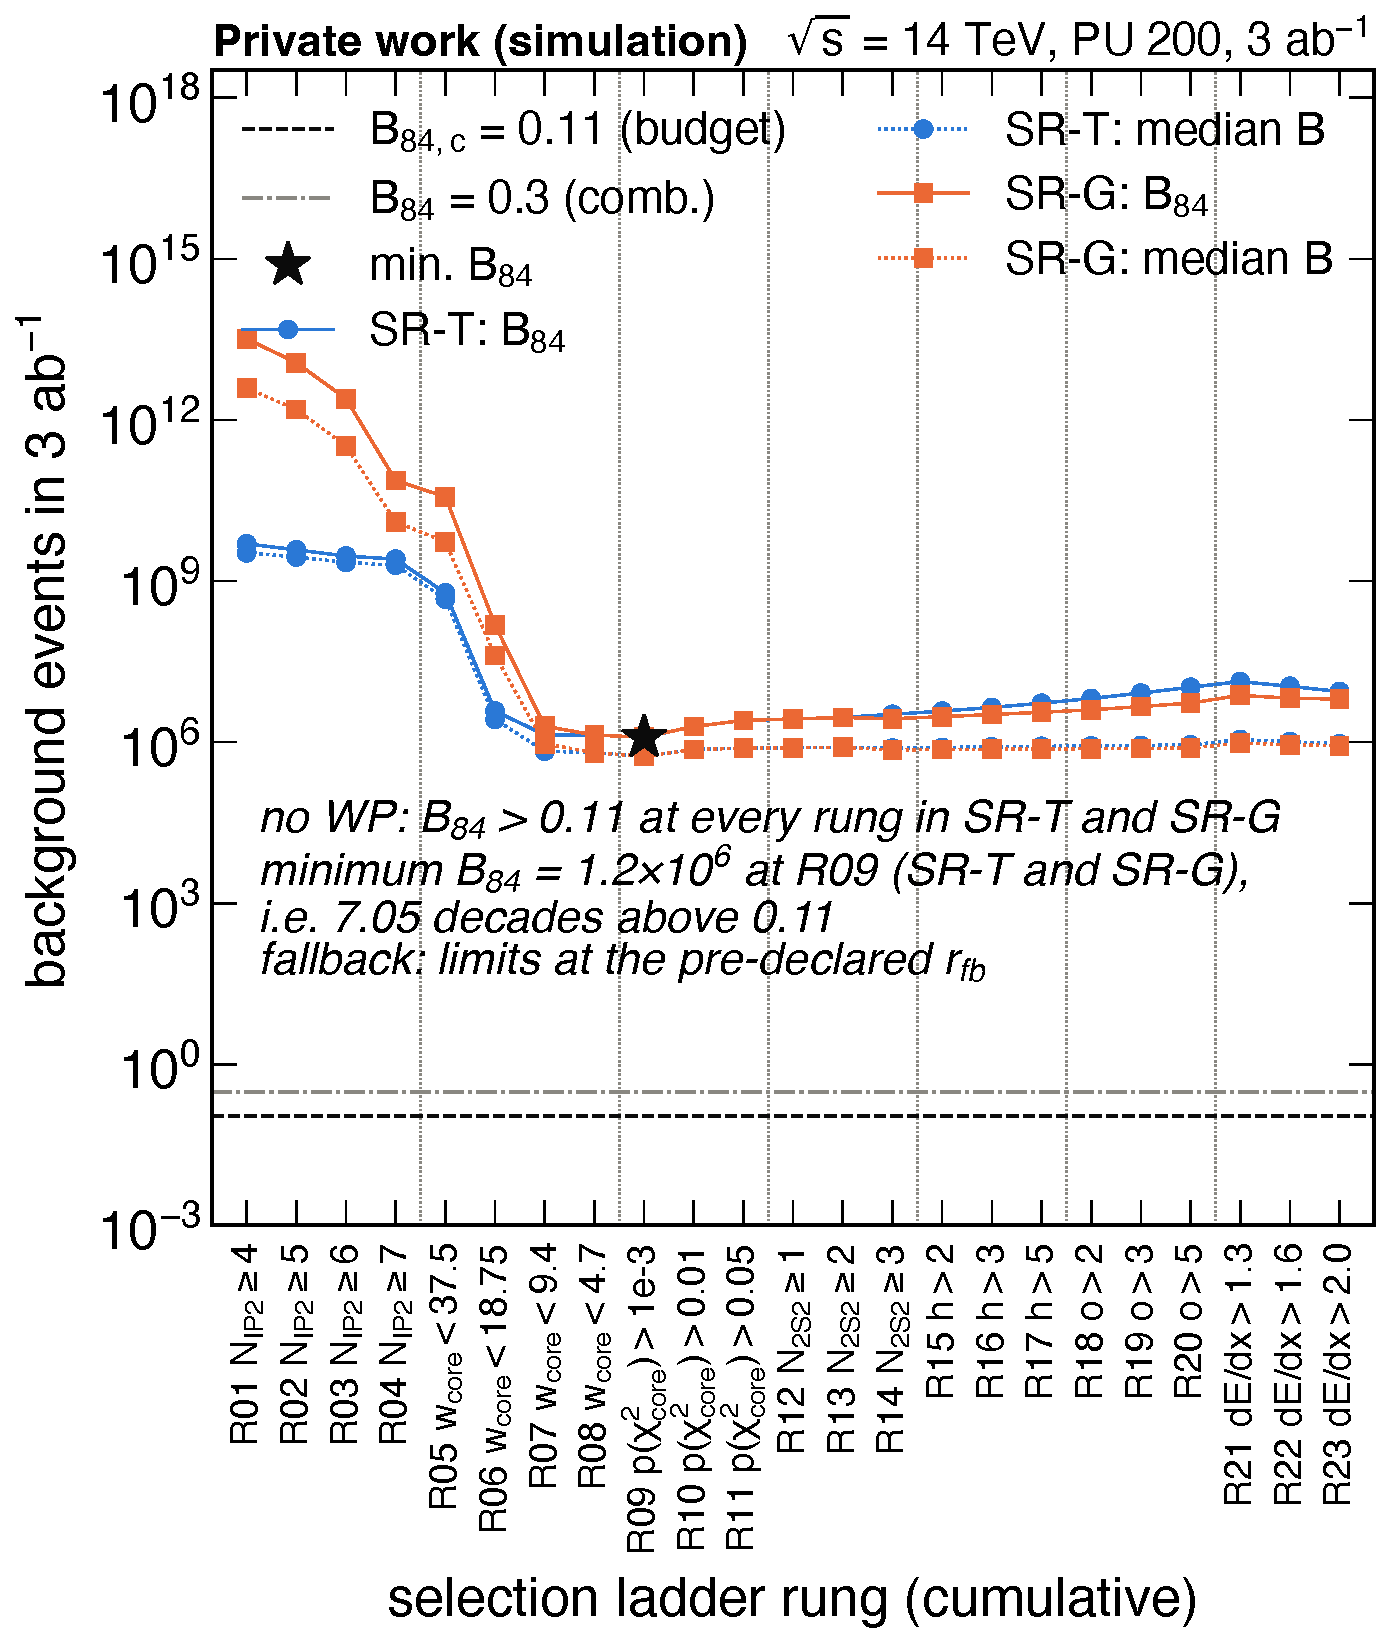
\includegraphics[height=0.37\linewidth]{figures/D3_bsum_vs_rung.pdf}\hspace{0.02\linewidth}
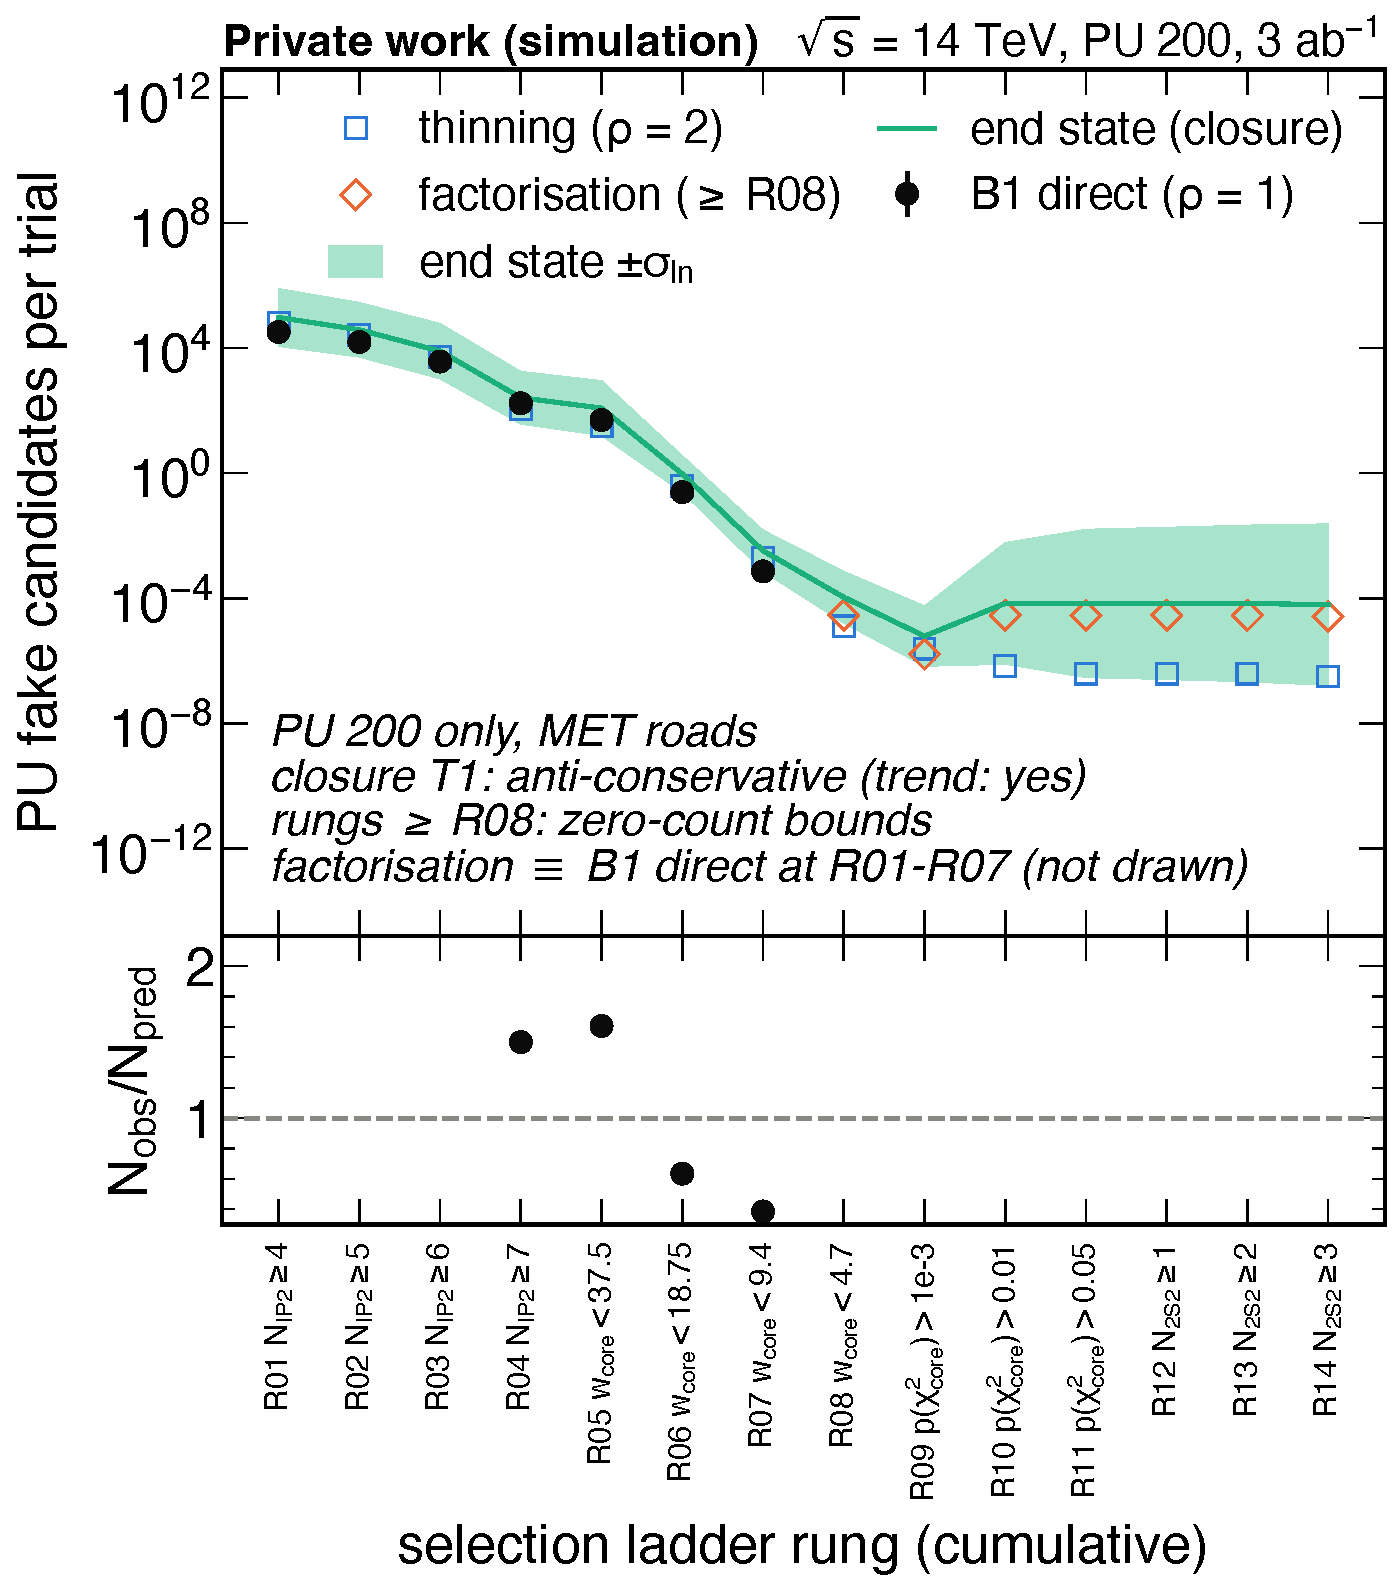
\includegraphics[height=0.37\linewidth]{figures/D4_pfake_extrapolation.pdf}
\caption{Background along the frozen ladder (detector level, PU 200, barrel). (Left) $\Nbkgeightyfour$ and the median
background in $3\abinv$ for SR-T and SR-G against the rung, with the per-category budget 0.11 and the combined 0.3; the
star marks the minimum, $1.2\times10^6$ at R09, 7.05 decades above the budget, so no working point exists. (Right)
Expected pile-up fake candidates per trial (one PU-200 event, one MET road): direct $\rho=1$ count, $\rho=2$ thinning,
the factorisation model where the direct count is zero, and the end state with the closure factor and its $\pm\sigma_{\ln}$
band; the lower panel shows the closure ratio $N_{\rm obs}/N_{\rm pred}$ at R04--R07. From R08 on the values are
zero-count bounds; the kink at R09--R10 comes from the switch between closure and extrapolation regimes.}
\label{fig:bkg}
\end{figure}

\paragraph{Why statistics alone cannot give a working point.} Each zero-count bound scales as $1/N$ with the sample
size. Bringing the leading bounded terms \emph{alone} to 0.11 would need $2.8\times10^9$ (PV pairs), $2.2\times10^9$
(decays in flight) and $8.4\times10^8$ ($Z(\nu\nu)$) events per sample, against 500--2000 now, and $\approx10^9$
$\rho=1$ trials for the pile-up term (now $4.8\times10^4$), whose irreducible trend and density uncertainty would still
require a median $\lesssim0.02$ (\EST{}). \textbf{The result is therefore limited by simulation statistics and by the
extrapolation uncertainty, not by a measured background}; a working point needs new handles or a data-driven background
estimate (Section~\ref{sec:concl}). Figure~\ref{fig:display} illustrates the difficulty: a pile-up-only fake can look as coplanar and as
non-helical in the transverse view as a quirk ribbon.

\begin{figure}[htbp]
\centering
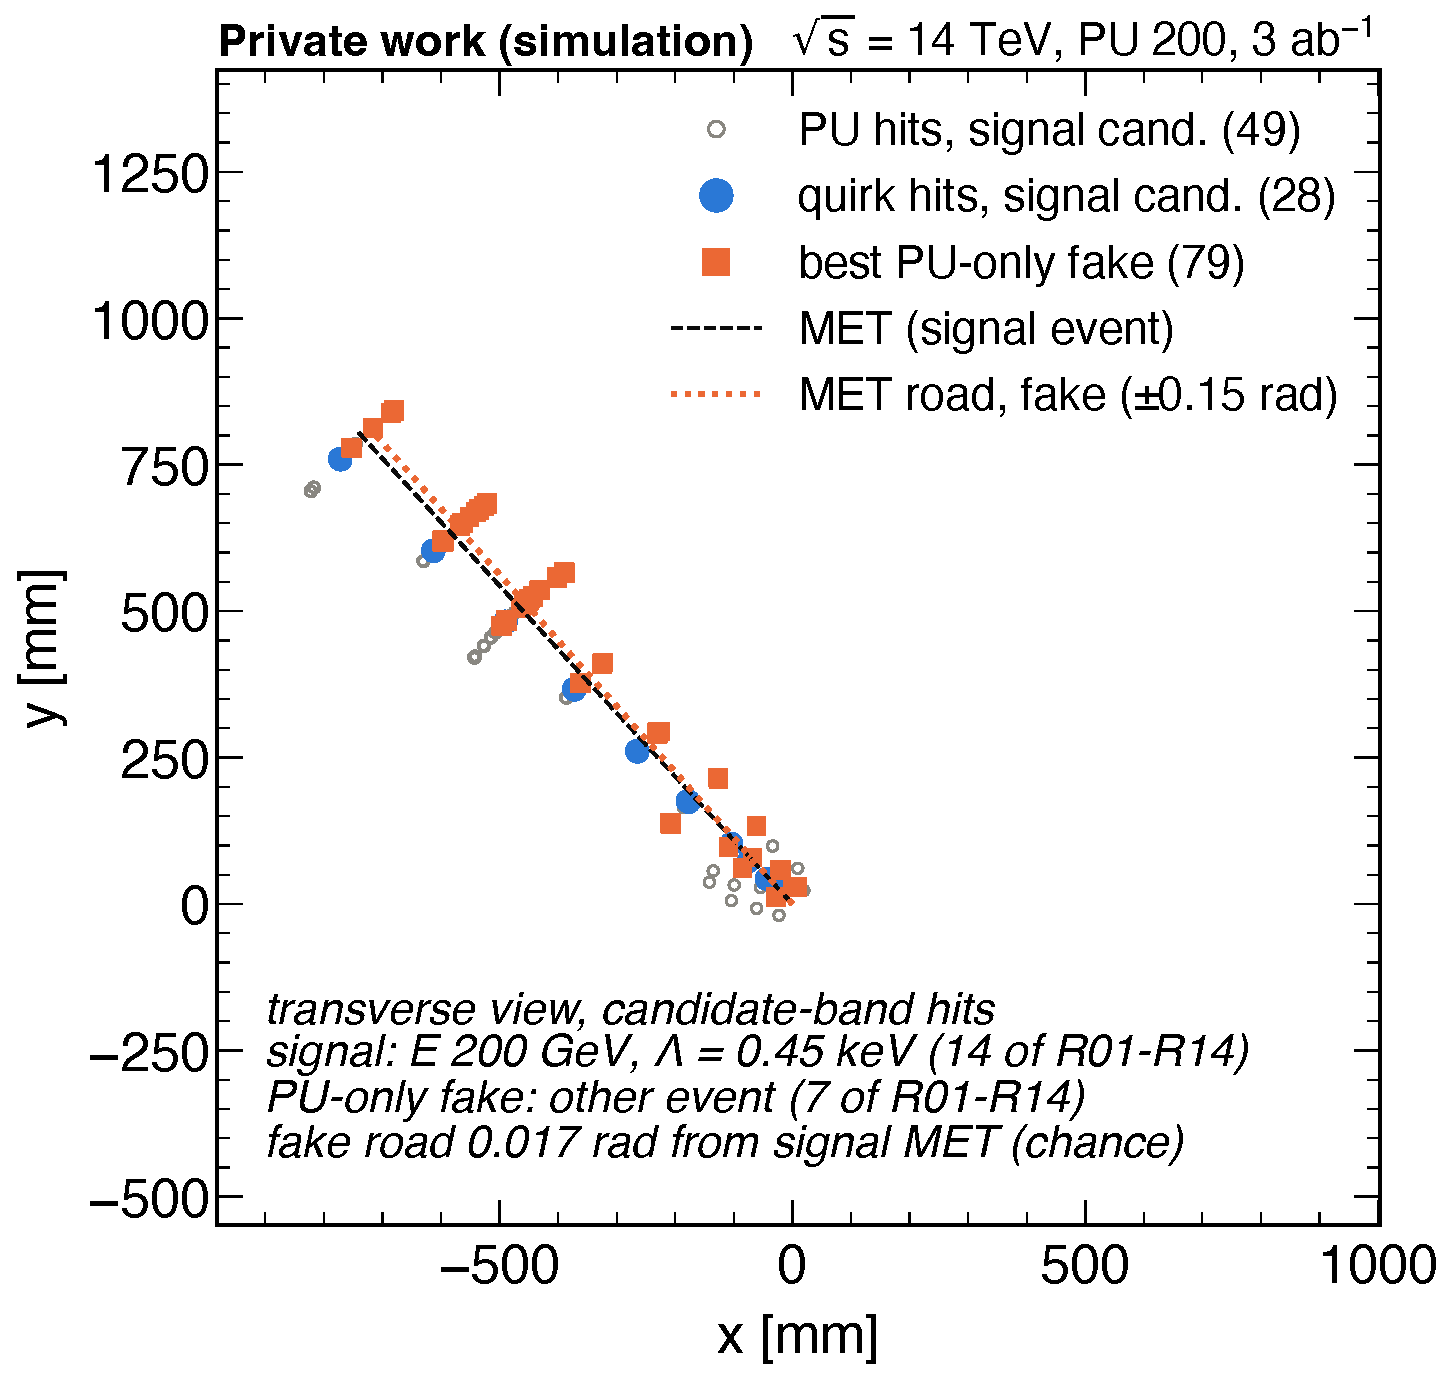
\includegraphics[height=0.32\linewidth]{figures/D11_event_display.pdf}
\caption{Transverse view of candidate-band hits at detector level (PU 200). Blue: quirk hits of a signal candidate ($E$ at
$200\GeV$, $\Lam=0.45\keV$, passing 14 of the rungs R01--R14), with the pile-up hits in its band (grey); orange: the best
pile-up-only fake of a different event (passing seven rungs), drawn in the same frame along its own MET road. Both lie along
a line through the vertex in this view; the fake fails the later width, core-$\chi^2$ and 2S rungs.}
\label{fig:display}
\end{figure}

